% !TEX root = ../main.tex

% 中英标题:\chapter{中文标题}[英文标题]
\chapter{后端轨迹生成算法设计}\label{chap:back_end_trajectory_generation}

\section{引言}\label{sec:intro_4}
上一章设计了轨迹规划的前端算法,
为本章所介绍的轨迹规划后端部分提供了数据输入。
后端部分的主要任务是根据前端生成的初始可行路径或安全飞行走廊,
通过拟合、优化的方法得到一条具备时间律的连续、平滑且安全的轨迹输入到飞行器的控制器中。
本章介绍基于优化的后端轨迹生成算法设计,
\ref{sec:geometrically_constrained_trajectory_optimization}节介绍几何约束下多旋翼的轨迹优化原理;
\ref{sec:geometrically_constrained_SE3_planning_for_omnihex}节基于该原理构建了几何约束下过驱动飞行器6自由度$SE(3)$轨迹优化框架,
并提出了该框架下使用欧拉角和使用四元数表示姿态的两种规划方式,并推导了相应公式。

\section{几何约束下多旋翼的轨迹优化原理}\label{sec:geometrically_constrained_trajectory_optimization}
几何约束下多旋翼的轨迹优化框架GCOPTER\cite{2021Geometrically}由Wang等人于2021年提出,
该框架在对多旋翼无人机施加复杂的安全约束、苛刻的动力学约束以及自定义需求的情况下依然能保证极高的计算效率和轨迹质量,
其优秀性能催生了许多优秀成果\cite{2021Fast, zhou2022swarm}。

GCOPTER论文的主要贡献概括为以下几点:
\begin{enumerate}
  \renewcommand{\labelenumi}{(\theenumi)}
  \item 给出了多阶段控制代价(control effort)最小化问题的最优充要条件,并基于此条件设计了最小控制代价轨迹类MINCO;
  \item 使用数学技巧消去轨迹时间分配的约束和中间点的空间空间约束;\label{itm:eliminate_geometric_constraints}
  \item 构造时间积分罚函数软化连续时间约束;\label{itm:time_int_penalty}
  \item 利用\ref{itm:eliminate_geometric_constraints}和\ref{itm:time_int_penalty}化约束优化问题为无约束优化问题,使用拟牛顿法(quasi-Newton methods)高效求解。
\end{enumerate}
本课题期望将此框架扩展到过驱动飞行器的6自由度$SE(3)$轨迹规划中,下面先对框架原理进行详细介绍。

\subsection{问题形式}\label{subsec:problem_formulation}
多旋翼无人机等微分平坦机器人的轨迹规划任务常常在其平坦输出空间中进行,
所期望得到的结果是一条平坦输出$\bm{z}$的轨迹$\bm{z}(t):[0, T]\mapsto\mathbb{R}^m$,
对于OmniHex这样的全驱动多旋翼飞行器而言有$m=6$。

GCOPTER的优化目标是在满足一定的几何约束和连续时间约束的前提下使轨迹尽量平滑且尽量满足设定的时间分配要求,
这个目标通过最小化时间正则化的导数平方积分控制代价来实现。
几何约束包括构型空间中的空间约束,代表飞行器可以处于的安全区域,表达为:
\begin{equation}
  \bm{z}(t) \in \mathcal{F}, \forall t \in  [0, T] \label{equ:spatial_constraints_in_c_space}
\end{equation}
其中$\mathcal{F}$为构型空间(平坦输出空间)中的无障碍物区域。
连续时间约束包含其他对飞行器状态$\bm{x}(t)$和控制输入$\bm{u}(t)$的所有约束,如动力学限制、其他与特定任务相关约束等。
所有这些自定义约束记为:
\begin{equation}
  \mathcal{G}_D(\bm{x}(t), \bm{u}(t)) \preceq \textbf{0}, \forall t \in [0, T]
  \label{equ:constraints_on_x_and_u}
\end{equation}
利用微分平坦关系可以将$\mathcal{G}_D$转化为对平坦输出及其有限阶导数的约束(\figref{fig:constraint_transformation}): 
\begin{equation}
  \mathcal{G}(\bm{z}(t), \dot{\bm{z}}(t), \cdots, \bm{z}^{(s)}(t)\}) \preceq \textbf{0}, \forall t \in [0, T]
  \label{equ:constraints_on_z}
\end{equation}
其中$\mathcal{G}$包含$n_g$个约束。

假设要最小化平方积分的导数阶数为$s \in \mathbb{N}_+$,
即取$\bm{v} = \bm{z}^{(s)}$,并记:
\begin{gather}
  \bm{z}^{[s-1]} = \trans{\left[\trans{\bm{z}} \  \trans{\dot{\bm{z}}} \  \cdots \trans{\bm{z}^{(s-1)}} \right]} \in \mathbb{R}^{ms} \label{equ:derivative_vector_of_z} \\
  \bm{z}_i^{[s-1]} = \trans{\left[ z_i \ \dot{z}_i \ \cdots z_i^{(s-1)} \right]} \in \mathbb{R}^{s} \label{equ:derivative_vector_of_zi}
\end{gather}
则整个轨迹优化过程即为求解下述约束优化问题:
\begin{subeqnarray}
  \label{equ:constrained_optimization}
  &\min_{\bm{z}(t), T} &\int_0^T \trans{\bm{v}(t)}\bm{v}(t)\text{d}t + \rho(T) \slabel{equ:time_regularized_control_effort} \\
  &s.t. &\bm{v}(t) = \bm{z}^{(s)}(t), \forall  t \in [0, T], \\
  & & \mathcal{G}(\bm{z}(t), \dot{\bm{z}}(t), \cdots, \bm{z}^{(s)}(t)\}) \preceq \textbf{0}, \forall t \in [0, T], \\
  & & \bm{z}(t) \in \mathcal{F}, \forall t \in  [0, T], \\ 
  & & \bm{z}^{[s-1]}(0) = \bar{\bm{z}}_o, \bm{z}^{[s-1]}(T) = \bar{\bm{z}}_f. \slabel{equ:boundary_conditions}
\end{subeqnarray}
其中$\rho(T)$为时间正则项,它代表了轨迹总时间所期望满足的性质,是控制代价与总时间之间的权衡。
例如,如果希望飞行器尽快到达重点,即总时间越$T$短越好,那么可取为$\rho_s(T) = k_\rho T$;
如果希望轨迹总时间尽可能接近给定的期望值$T_{\Sigma}$,那么可取为$\rho_s(T) = k_\rho (T - T_{\Sigma})^2$;
如果希望$T$严格固定为$T_{\Sigma}$,则可取为:
\begin{equation}
  \rho_f(T) = 
  \begin{cases}
    0 \quad &if \  T = T_{\Sigma} \\
    \infty \quad &if \ T \neq T_{\Sigma}
  \end{cases}
  \label{equ:fixed_time_regularization_term}
\end{equation}

\subsection{最优性条件与MINCO轨迹类}\label{subsec:optimal_condition_and minco_trajectory}
为了使轨迹更容易地满足安全约束和动力学约束,通常将平坦输出轨迹$\bm{z}(t)$表示为分段多项式,
一条$k$阶$M$段分段多项式轨迹形式如下:
\begin{equation}
  \bm{z}(t) = \trans{\bm{c}_i}\bm{\beta}(t - t_{i-1}), t \in [t_{i-1}, t_i], i = 1, 2, \cdots, M
  \label{equ:piecewise_polynomial_trajectory} 
\end{equation}
其中$\bm{c}_i \in \mathbb{R}^{(k+1) \times m}$为第$i$段多项式的系数矩阵,
$\bm{\beta}(t) = \left[1 \  t \  \cdots \  t^N\right] \in \mathbb{R}^{(k+1)}$为多项式基底。

先不考虑约束$\mathcal{F}$和$\mathcal{G}$以及时间正则项$\rho(T)$,考虑如下$M$阶段控制代价最小化问题:
\begin{subeqnarray}
  \label{equ:unconstrained_multistage_optimal_control_problem}
  &\min_{\bm{z}(t)} &\int_{t_0}^{t_M} \trans{\bm{v}(t)}\bm{v}(t)\text{d}t \slabel{equ:control_effort} \\
  &s.t. &\bm{v}(t) = \bm{z}^{(s)}(t), \forall t \in [t_0, t_M], \\
  & & \bm{z}^{[s-1]}(0) = \bar{\bm{z}}_o, \bm{z}^{[s-1]}(T) = \bar{\bm{z}}_f, \slabel{equ:intermediate_conditions_moc}\\
  & & \bm{z}^{[d_i-1]}(t_i) = \bar{\bm{z}}_i, i = 1, 2, \cdots, M-1, \slabel{equ:boundary_conditions_moc}\\
  & & t_{i-1} < t_i, i = 1, 2, \cdots, M. \slabel{equ:temporal_non_negative_constraints}
\end{subeqnarray}
在这个问题中,时间段$[t_0, t_M]$被$(M+1)$个固定的时间戳$ t_1, \cdots, t_{M-1}  $分割成$M$段;
此外,在每段的终点$t_i$处平坦输出的前$d_i - 1 < s$阶导数也被固定为$\bm{z}_i \in \mathbb{R}^{md_i}$。
在GCOPTER的论文中给出了多阶段最优控制问题\equref{equ:unconstrained_multistage_optimal_control_problem}的最优充要条件:
\begin{theorem}[(最优充要条件)]
  \label{thr:optimality_conditions}
  优化问题\equref{equ:unconstrained_multistage_optimal_control_problem}存在唯一一个最优解$\bm{z}^*(t):[t_0, t_M] \mapsto \mathbb{R}^m$;
  且轨迹$\bm{z}$是优化问题\equref{equ:unconstrained_multistage_optimal_control_problem}的最优解,
  当且仅当如下条件同时成立:
  \begin{enumerate}
    \renewcommand{\labelenumi}{(\theenumi)}
    \item $\bm{z}^*(t):[t_0, t_M] \mapsto \mathbb{R}^m$是一个$(2s-1)$次多项式,$1 \leq i \leq M$;
    \item $\bm{z}^*(t)$满足\equref{equ:boundary_conditions_moc}所示的边界条件;
    \item $\bm{z}^*(t)$满足\equref{equ:intermediate_conditions_moc}所示的中间条件;
    \item 对任意的$i = 1, \cdots, M-1$,$\bm{z}^*(t)$在$t_i$处$\bar{d}_i-1$阶连续可微,其中处$\bar{d}_i=2s-d_i$。
  \end{enumerate}
\end{theorem}
利用这个最优充要条件,就可以无需计算代价泛函,以$O(M)$的时间复杂度求出这条最优轨迹。

记\equref{equ:unconstrained_multistage_optimal_control_problem}的最优轨迹$\bm{z}^*(t)$的总系数矩阵为;
\begin{equation}
  \bm{c} = \trans{
    \begin{bmatrix}
      \trans{\bm{c}_1} & \cdots & \trans{\bm{c}_1}
    \end{bmatrix}
  } \in \mathbb{R}^{2Ms \times m}
  \label{equ:coeff_matrix_of_the_whole_traj} 
\end{equation}
时间分配向量记为:
\begin{equation}
  \bm{T} = \trans{
    \begin{bmatrix}
      t_1 - t_0 & \cdots & t_M - t_{M-1}
    \end{bmatrix}
  } = \trans{
    \begin{bmatrix}
      T_1 & \cdots & T_M
    \end{bmatrix}
  } \in \mathbb{R}_+^{M}
  \label{equ:time_alloc_vector}
\end{equation}
记\equref{equ:unconstrained_multistage_optimal_control_problem}中的边界条件为$\bm{D}_0, \bm{D}_M \in \mathbb{R}^{s \times m}$,
中间条件为$\bm{D}_i \in \mathbb{R}^{d_i \times m}$,
这样根据定理\ref{thr:optimality_conditions}中关于中间时刻$t_i$处导数的取值条件和连续性条件可以写为下式:
\begin{equation}
  \begin{bmatrix}
    \bm{E}_i & \bm{F}_i
  \end{bmatrix}
  \begin{bmatrix}
    \bm{c}_i \\ \bm{c}_{i+1}
  \end{bmatrix} =
  \begin{bmatrix}
    \bm{D}_i \\ \textbf{0}_{\bar{d}_i \times m}
  \end{bmatrix}, 
  i = 1, 2, \cdots, M-1
  \label{equ:conditons_at_t_i}
\end{equation}
其中$E_i,F_I \in \mathbb{R}^{2s \times 2s}$,且有:
\begin{gather}
  \bm{E}_i = \trans{
    \begin{bmatrix}
      \bm{\beta}(T_i) & \cdots & \bm{\beta}^{(d_i-1)}(T_i) & \bm{\beta}(T_i) & \cdots & \bm{\beta}^{(\bar{d}_i-1)}(T_i)
    \end{bmatrix}
  } \label{equ:E_i}\\
  \bm{F}_i = \trans{
    \begin{bmatrix}
      \textbf{0} & -\bm{\beta}(0) & \cdots & -\bm{\beta}^{(\bar{d}_i-1)}(0)
    \end{bmatrix}
  }
  \label{equ:F_i}
\end{gather}
特别地,定义$\bm{F}_0,\bm{E}_M \in \mathbb{R}^{s \times 2s}$为:
\begin{gather}
  \bm{F}_0 = \trans{
    \begin{bmatrix}
      \bm{\beta}(0) & \cdots & \bm{\beta}^{(s-1)}(0)
    \end{bmatrix}
  } \label{equ:F_0}\\
  \bm{E}_M = \trans{
    \begin{bmatrix}
      \bm{\beta}(T_M) & \cdots & \bm{\beta}^{(s-1)}(T_M)
    \end{bmatrix}
  }
  \label{equ:E_M}
\end{gather}
于是,根据定理\ref{thr:optimality_conditions}可构造出关于最优轨迹系数矩阵$\bm{c}$的线性方程组:
\begin{equation}
  \bm{Mc} = \bm{b}
  \label{equ:linear_equation_system_wrt_c}
\end{equation}
其中$\bm{M} \in \mathbb{R}^{2Ms \times 2Ms}$仅与时间分配向量$\bm{T}$有关,具有带状结构;
$\bm{b} \in \mathbb{R}^{2Ms \times m}$仅与中间条件有关。
二者形式如下:
\begin{gather}
  \bm{M} = 
    \begin{bmatrix}
      \bm{F}_0 & \textbf{0} & \textbf{0} & \cdots & \textbf{0} \\
      \bm{E}_1 & \bm{F}_1 & \textbf{0} & \cdots & \textbf{0} \\
      \textbf{0} & \bm{E}_2 & \bm{F}_2 & \cdots & \textbf{0} \\ 
      \vdots & \vdots & \vdots & \ddots & \vdots \\
      \textbf{0} & \textbf{0} & \textbf{0} & \cdots & \bm{F}_{M-1} \\
      \textbf{0} & \textbf{0} & \textbf{0} & \cdots & \bm{E}_{M}
    \end{bmatrix}
   \label{equ:M} \\
  \bm{b} = \trans{
    \begin{bmatrix}
      \bm{D}_0^{\text{T}} & \bm{D}_1^{\text{T}} & \textbf{0}_{m \times \bar{d}_i} & 
      \cdots & \bm{D}_{M-1}^{\text{T}} & \textbf{0}_{m \times \bar{d}_{M-1}} & \bm{D}_{M}^{\text{T}}
    \end{bmatrix}
  } \label{equ:b}
\end{gather}

由最优解的存在性和唯一性,可以保证$\bm{M}$的非奇异性,
然后利用带状矩阵的PLU分解就可以以$O(M)$的线性时间和空间复杂度求解出$\bm{c}$;
同时对任意的时间分配、边界条件和中间条件,$\bm{M}$和$\bm{b}$均可以以线性复杂度构建。
这样,通过直接应用定理\ref{thr:optimality_conditions},
无需代价泛函即可用极低的复杂度得到多阶段最优控制问题\equref{equ:unconstrained_multistage_optimal_control_problem}的最优解。
需要注意的是,
如果在算法实现时采用的时直接LU分解,那么需要调整$\bm{M}$和$\bm{b}$中行的顺序来避免主对角线上出现0。

对于多旋翼飞行器来说,飞行轨迹的安全性通常决定于它的空间特性,而动力学限制通常决定于它的时间属性,
因此将轨迹参数分为两组:
第一组包含轨迹必须通过的中间点;第二组包含轨迹中不同片段的时间分配向量。
基于这些参数,利用定理\ref{thr:optimality_conditions}即可得到轨迹的系数矩阵$\bm{c}$,
这个系数矩阵对应的就是在给定的阶数、时间分配和中间条件下具有最小控制量的轨迹,
若$s=4$,那么得到的就是Mellinger等人提出的最小化加加加速度轨迹\cite{2011minimumsnap}.
Wang等人将这类以中间点和时间分配为参数,使用定理\ref{thr:optimality_conditions}构建出的轨迹称作MINCO轨迹\cite{2021Geometrically}。

记中间点为$\bm{q} = \begin{bmatrix} \bm{q}_1 & \cdots & \bm{q}_{M-1} \end{bmatrix} \in \mathbb{R}^{m \times (M-1)}$,
$\bm{q}_i \in \mathbb{R}^m$为指定在$t_i$时刻的中间条件($d_i-1=0$),
则MINCO轨迹定义为$\mathscr{T}_{\text{MINCO}}$定义为
\begin{equation}
  \mathscr{T}_{\text{MINCO}} \overset{\text{def}}{=} 
  \{
    \bm{p}(t):[t_0, t_M] \mapsto \mathbb{R}^m \mid \bm{c} = \bm{c}(\bm{q}, \bm{T}), \forall \bm{q} \in \mathbb{R}^{m \times (M-1)}, \bm{T} \in \mathbb{R}_+^{M}
  \}
  \label{equ:definition_of_minco}
\end{equation}
其中$\bm{c}(\bm{q}, \bm{T})$即是由定理\ref{thr:optimality_conditions}决定的整条轨迹的系数矩阵,
这样轨迹的参数就由系数转化为了$\bm{q}$和$\bm{T}$,实现了参数降维.

\begin{figure}[ht]
  \centering
  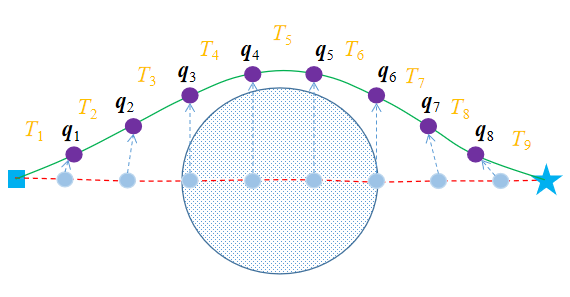
\includegraphics[width = 0.58\textwidth]{minco.png}
  \caption{MINCO轨迹的空间变形示意图}
  \label{fig:minco}
\end{figure}

现在如果有约束存在,
则调整$\bm{q}$就可以对$\mathscr{T}_{\text{MINCO}}$进行空间上的变形,使整条轨迹不与障碍物发生碰撞(\figref{fig:minco});
调整$\bm{T}$则可以对$\mathscr{T}_{\text{MINCO}}$进行时间上的变形,使之满足动力学限制。
GCOPTER框架就是通过MINCO的时空变形来优化目标函数,从而得到一条给定需求下的最优轨迹。

\subsection{MINCO轨迹类中的梯度计算}\label{subsec:gradient_calculation_in_minco}
上小节提到,基于MINCO的轨迹优化框架通过调整轨迹参数$\bm{q}$和$\bm{T}$来优化给定的目标函数。
及自定义的轨迹优化优化目标函数为一个二阶连续可微的标量函数$F(\bm{c}, \bm{T})$,且其梯度已知,
那么这个目标函数在$\mathscr{T}_{\text{MINCO}}$中可以计算如下:
\begin{equation}
  H(\bm{q}, \bm{T}) = F(\bm{c}(\bm{q}, \bm{T}), \bm{T})
  \label{equ:objective_form_in_minco}
\end{equation}

在对目标函数进行优化时,通常需要用到其梯度信息,
即需要计算${\partial H}/{\partial \bm{q}}$和${\partial H}/{\partial \bm{T}}$。
显然计算$H$的值与求解$\mathscr{T}_{\text{MINCO}}$中任意一条轨迹(即计算$\bm{c}(\bm{q}, \bm{T})$)具有相同的复杂度$O(M)$,
下面介绍从已知的${\partial F}/{\partial \bm{c}}$和${\partial F}/{\partial \bm{T}}$计算${\partial H}/{\partial \bm{q}}$和${\partial H}/{\partial \bm{T}}$的线性复杂度方法。

首先给出如下结论,这里省去推导过程:
\begin{equation}
  \pdiff{H}{\bm{q}_i} = \trans{\left(\bm{M}^{-\text{T}}\pdiff{F}{\bm{c}}\right)} \bm{e}_{(2i-1)s+1}
  \label{equ:grad_H_qi}
\end{equation}
其中$\bm{e}_j$代表单位矩阵$\bm{I}_{2Ms}$的第$j$列。
计算过程中需要对$\trans{\bm{M}}$求逆,直接的求逆运算具有$O(M^3)$的时间复杂度。
注意到先前求解$\bm{c}$时对$\bm{M}$进行了PLU分解,可以利用这里的结果来避免求逆,减小复杂度。
令\equref{equ:grad_H_qi}中括号中表达式的结果为$\bm{G}\in\mathbb{R}^{2Ms\times m}$,
则得到关于$\bm{G}$的线性方程组: 
\begin{equation}
  \trans{\bm{M}}\bm{G} = \pdiff{F}{\bm{c}}
  \label{equ:linear_equation_system_wrt_G}
\end{equation}
记$M$的PLU分解结果为$\bm{M} = \bm{PLU}$,则$\trans{\bm{M}}$也存在PLU分解,有$\trans{\bm{M}}=\bar{\bm{L}}\bar{\bm{U}}\trans{\bm{P}}$,其中 
\begin{equation}
  \bar{\bm{L}} = \trans{\bm{U}}(\bm{U}\circ\bm{I})^{-1}, \bar{\bm{U}} = (\bm{U}\circ\bm{I})\trans{\bm{L}}
  \label{equ:LU_of_trans_M}
\end{equation}
其中需要求逆的只是一个对角矩阵,符号$\circ$为矩阵的Hadamard乘积。
那么现在就可以用线性复杂度求出$\bm{G}$了,
为方便起见,将$\bm{G}$写成如下分块形式:
\begin{equation}
  \bm{G} = \trans{
    \begin{bmatrix}
      \bm{G}_0^{\text{T}} & \bm{G}_1^{\text{T}} & \cdots & \bm{G}_{M-1}^{\text{T}} & \bm{G}_M^{\text{T}}
    \end{bmatrix}
  }
  \label{equ:block_form_of_G}
\end{equation}
其中$\bm{G}_0, \bm{G}_M \in \mathbb{R}^{s \times m}$而$\bm{G}_i \in \mathbb{R}^{2s \times m}, i = 1, 2, \cdots, M-1$。
这样$H$对$\bm{q}$的梯度就可以写为:
\begin{equation}
  \pdiff{H}{\bm{q}} = 
  \begin{bmatrix}
    \bm{G}_1^{\text{T}}\bm{e}_1 & \cdots & \bm{G}_{M-1}^{\text{T}}\bm{e}_1
  \end{bmatrix}
  \label{equ:grad_H_q}
\end{equation}
相似地可以得到$H$对$T_i$的梯度: 
\begin{equation}
  \pdiff{H}{T_i} = \pdiff{F}{T_i} - \text{tr}\{\bm{G}_i^{\text{T}}\pdiff{\bm{E}_i}{T_i}\bm{c}_i\}
  \label{equ:grad_H_Ti}
\end{equation}

\subsection{几何约束的消去}\label{subsec:elimination_of_geometric_constraints}
在MINCO轨迹类中,进行时空变形可使轨迹在满足可行性约束的同时保持局部光滑性。
基于$\mathscr{T}_{\text{MINCO}}$的轨迹优化问题的形式如下:
\begin{subeqnarray}
  \label{equ:optimization_in_minco}
  &\min_{\bm{q}, \bm{T}} &J(\bm{q}, \bm{T}) = J_q(\bm{q}, \bm{T}) + \rho(\Vert\bm{T}\Vert_1) \slabel{equ:time_regularized_control_effort_in_minco} \\
  &s.t. \ &\mathcal{G}(\bm{z}(t), \dot{\bm{z}}(t), \cdots, \bm{z}^{(s)}(t)) \preceq \textbf{0}, \forall t \in [0, T], \slabel{equ:time_continuos_constraint_minco}\\
  & & \bm{q}_i \in \mathcal{P}_i, i = 1, 2, \cdots, M-1, \slabel{equ:spatial_constraints_minco}\\ 
  & & \bm{T} \succ \textbf{0}, \slabel{equ:temporal_constraints_minco}\\
  & & \bm{z}^{[s-1]}(0) = \bar{\bm{z}}_o, \bm{z}^{[s-1]}(T) = \bar{\bm{z}}_f. \slabel{equ:boundary_conditions_minco}
\end{subeqnarray}
其中$J_q(\bm{q}, \bm{T}):=J_c(\bm{c}, \bm{T})$,$J_c(\bm{c}, \bm{T})$为由轨迹多项式系数和时间分配确定的控制代价,
具有解析的表达式和梯度\cite{2021Geometrically};$\mathcal{P}_i$为第$i$个中间点$\bm{q}_i$所被分配到的SFC凸多面体。

几何约束\equref{equ:spatial_constraints_minco}和\equref{equ:temporal_constraints_minco}是必要的,
但会在一定程度上影响优化速度
下面介绍消去几何约束使时空变形免受不等式约束组合困难(combinatorial difficulty)的限制的方法。
\subsubsection{时间约束的消去}\label{subsubsec:elimination_of_temporal_constraints}
对时间分配向量$\bm{T}$的两种约束会对带约束优化过程产生不利影响:
\begin{enumerate}
  \renewcommand{\labelenumi}{(\theenumi)}
  \item 如\equref{equ:temporal_constraints_minco}所示的那样,要求$\bm{T}$中的每个元素都大于0,
        这是由实际意义决定的,并且如\figref{fig:influence_of_temporal_constraints}所示,当
        $\bm{T}$中的任意一个元素在优化过程中接近于0时,都会导致$J_q$趋向于无穷大,因为$\bm{q}$中不存在两个相邻且相同的点;
  \item 如\figref{fig:influence_of_temporal_constraints}所示, 
        当$\rho=\rho_f$时,会加入一个额外的约束$\sum_{i = 1}^{M-1}T_i < T_{\Sigma}$,使得$\bm{T}$的可行区域进一步缩减。
\end{enumerate}

在上述两种情况下,病态的Hessian矩阵以及可行域边界处出现的不可行搜索步长都会拖慢优化过程的收敛。
在GCOPTER中,采取微分同胚映射(diffeomorphism)的手段来消去上述时间约束。
\begin{figure}[ht]
  \centering
  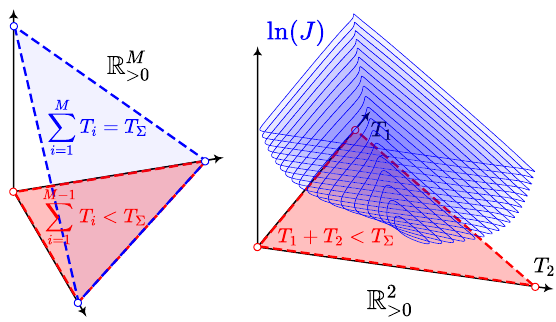
\includegraphics[width = 0.58\textwidth]{influence_of_temporal_constraints.png}
  \caption{时间约束示意图}
  \label{fig:influence_of_temporal_constraints}
\end{figure}

对于要求总时间严格固定,即$\rho=\rho_f$的情形,$\bm{T}$的可行域描述为如下集合:
\begin{equation}
  \mathcal{T}_f = \{
    \bm{T} \in \mathbb{R}_+^M \mid \Vert\bm{T}\Vert_1 = T_{\Sigma}
  \}
  \label{equ:feasible_domain_of_T_fixed_tt}
\end{equation}
那么可以证明$\mathcal{T}_f$与$\mathbb{R}^{M-1}$是微分同胚的,
其中一个$C^{\infty}$的微分同胚映射如\equref{equ:diffeophism_T_fixed_tt}所示
\begin{subeqnarray}
  \label{equ:diffeophism_T_fixed_tt}
  &T_i = \frac{e^{\tau_i}}{1 + \sum_{j=1}^{M-1}e^{\tau_j}}T_{\Sigma}, i = 1, 2, \cdots, M-1, \slabel{equ:diffeophism_T_fixed_tt_1} \\ 
  &T_M = T_{\Sigma} - \sum_{i=1}^{M-1}T_i \slabel{equ:diffeophism_T_fixed_tt_2}
\end{subeqnarray}
利用这个映射,把目标变量由受约束的$\bm{T}$转化为自由变量$\bm{\tau}$,
这样就摆脱了可行域边界附近的不利条件,且此时时间正则项恒为0。
若令${\partial J_q}/{\partial \bm{T}} = [\bm{g}_a^{\text{T}} \  g_b]^{\text{T}}$,
则$J$对$\bm{\tau}$的梯度如下式所示:
\begin{equation}
  \pdiff{J}{\bm{\tau}} = 
  \left(
  \frac{(\bm{g}_a - g_b \cdot \textbf{1}) \circ e^{[\bm{\tau}]}}{1 + \Vert e^{[\bm{\tau}]} \Vert_1} - 
  \frac{(\bm{g}_a^{\text{T}}e^{[\bm{\tau}]} - g_b\Vert e^{[\bm{\tau}]} \Vert_1)e^{[\bm{\tau}]}}{(1 + \Vert e^{[\bm{\tau}]} \Vert_1)^2}
  \right)T_{\Sigma}
  \label{equ:grad_J_tau}
\end{equation}
其中$e^{[\cdot]}$表示向量$\cdot$按元素求指数函数值。
那么可以看到,由$\bm{\tau}$正向计算$J$以及反向计算梯度仍然只需要$O(M)$的时间和空间复杂度。
对于总时间不严格固定,即$\rho=\rho_s$的情形,
可以用$\bm{T}=e^{[\bm{\tau}]}$作为从$\mathbb{R}^M$到作为从$\mathbb{R}_+^M$的微分同胚映射,
注意此时在计算目标函数值和梯度时需要加上时间正则项。

可以证明,上述变换不会抹去$J$原有的局部最小值点,也不会引入额外的局部最小值点。

\subsubsection{空间约束的消去}\label{subsubsec:elimination_of_spatial_constraints}
对于\equref{equ:spatial_constraints_in_c_space}所示的空间约束,
要求对整条轨迹上的点都成立。
对于由凸多面体组成的复杂空间约束,这个要求通过两个阶段来实现:
(1)按顺序将中间点分配到组成安全飞行走廊的凸多面体中,如\equref{equ:spatial_constraints_minco}所示;
(2)在给定分辨率下使整条轨迹满足空间约束。
本小节处理阶段(1),阶段(2)的处理将在\ref{subsec:processing_of_continuous_time_constraints}小节介绍。

\begin{figure}[ht]
  \centering
  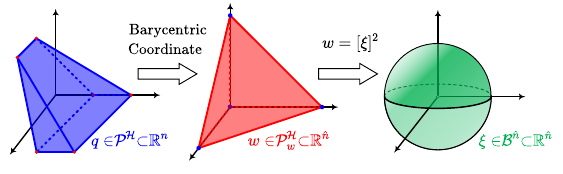
\includegraphics[width = 0.7\textwidth]{polyhedron_constraint_elimination.png}
  \caption{凸多面体约束转化示意图}
  \label{fig:transformation_of_polyhedron_constraints}
\end{figure}

记一个$\mathbb{R}^n$中的凸多面体$\mathcal{P}$的$(\hat{n}+1)$个顶点为$[\bm{v}_0 \ \cdots \ \bm{v}_{\hat{n}}]$,
记$\hat{\bm{v}}_i = \bm{v}_i - \bm{v}_0$,及$\hat{\bm{V}} = [\hat{\bm{v}}_1 \ \cdots \ \hat{\bm{v}}_{\hat{n}}]$,
这样每一个中间点$\bm{q}\in\mathbb{R}^n$在重心坐标系(barycentric coordinate system)下就可以表示为:
\begin{equation}
  \bm{q} = \bm{v}_0 + \hat{\bm{V}}\bm{w}
  \label{equ:q_in_barycentric_coordinate}
\end{equation}
其中$\bm{w} = \trans{[w_1 \ \cdots \ w_{\hat{n}}]}\in\mathbb{R}^{\hat{n}}$为重心坐标的后$\hat{n}$个元素。
凸多面体$\mathcal{P}$内的每一个点对应的$\bm{w}$构成的点集是$\mathbb{R}^{\hat{n}}$中的标准单纯形(standard simplex):
\begin{equation}
  \mathcal{P}_w^{\hat{n}} = \{
    \bm{w} \in \mathbb{R}^{\hat{n}} \mid \bm{w} \succeq \textbf{0}, \Vert \bm{w} \Vert_1 \leq 1
  \}
  \label{equ:standard_simplex}
\end{equation}
这样凸多面体$\mathcal{P}$就可以用V-表示法表达为:
\begin{equation}
  \mathcal{P} = \{
    \bm{v}_0 + \hat{\bm{V}}\bm{w} \mid \bm{w} \in \mathcal{P}_w^{\hat{n}}
  \}
  \label{equ:V_polyhedron}
\end{equation}

换句话说,凸多面体约束$\bm{q} \in \mathcal{P}$实际上被转化为了一个$\mathbb{R}^{\hat{n}}$中的标准单纯形约束$\bm{w} \in \mathcal{P}_w^{\hat{n}}$(\figref{fig:transformation_of_polyhedron_constraints})。
此单纯形约束还可以进一步用非线性变换消去:
首先用按元素的平方变换$\bm{w}=[\bm{x}]^2,\forall x\in\mathbb{R}^{\hat{n}}$消去非负约束,
这样单纯形约束$\bm{w} \in \mathcal{P}_w^{\hat{n}}$转化为了球约束$\bm{x}\in\mathcal{B}^{\hat{n}}$,其中:
\begin{equation}
  \mathcal{B}^{\hat{n}} = \{ 
    \bm{x} \in \mathbb{R}^{\hat{n}} \mid \Vert \bm{x} \Vert_2 \leq 1
  \}
  \label{equ:ball_constraint}
\end{equation}
\begin{figure}[ht]
  \centering
  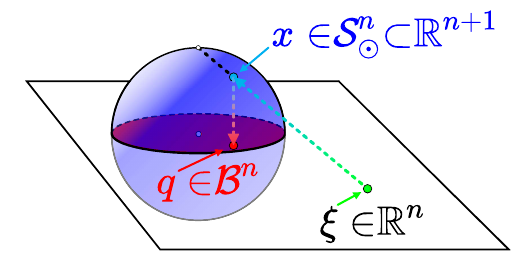
\includegraphics[width = 0.62\textwidth]{ball_constraint_elimination.png}
  \caption{球约束消去示意图}
  \label{fig:elimination_of_ball_constraints}
\end{figure}
然后再如\figref{fig:elimination_of_ball_constraints}所示使用逆球极投影(inverse stereographic projection)变换和一个正交投影变换可以消去球约束,
最后得到一个从整个$\mathbb{R}^{\hat{n}}$到凸多面体$\mathcal{P}$的映射:
\begin{equation}
  f_{\mathcal{H}}(\bm{\xi}) = \bm{v}_0 + \frac{4\hat{\bm{V}}[\bm{\xi}]^2}{(\trans{\bm{\xi}}\bm{\xi} + 1)^2} \in \mathcal{P}, 
  \forall \bm{\xi} \in \mathbb{R}^{\hat{n}}
  \label{equ:polyhedron_constraint_elimination_map}
\end{equation}
当$\bm{\xi}$在整个$\mathbb{R}^{\hat{n}}$中自由运动时,
经由映射$f_{\mathcal{H}}$得到的$\mathbb{R}^n$中的像始终位于凸多面体$\mathcal{P}$内。
这样,与时间约束类似,用凸多面体表示的空间约束被用引入新的目标变量$\bm{\xi}$的方式消去了。
在优化过程开始之前会给定的初始$\bm{q}_i$,其对应的初始$\bm{\xi}_i$可以通过最小化$\Vert \bm{f}_{\mathcal{H}}(\bm{\xi}_i) - \bm{q}_i \Vert_2^2$的值来得到。


若记${\partial J}/{\partial \bm{q}_i}=\bm{g}_i$,则$J$关于对应的$\bm{\xi}_i$的梯度就可以写为:
\begin{equation}
  \pdiff{J}{\bm{\xi}_i} = 
  \frac{8\bm{\xi}_i \circ \trans{\hat{\bm{V}}}\bm{g}_i}{(\bm{\xi}_i^{\text{T}}\bm{\xi}_i+1)^2} - 
  \frac{16\bm{g}_i^{\text{T}}\hat{\bm{V}}[\bm{\xi}]^2}{(\bm{\xi}_i^{\text{T}}\bm{\xi}_i+1)^3}\bm{\xi}_i
  \label{equ:grad_J_xii}
\end{equation}

上述变换同样不会抹去$J$原有的局部最小值点,也不会引入额外的局部最小值点。

\subsection{连续时间约束$\mathcal{G}$的处理}\label{subsec:processing_of_continuous_time_constraints}
\equref{equ:time_continuos_constraint_minco}表达的连续时间$\mathcal{G}$约束包含无穷多个不等式约束,计算机难以处理。
GCOPTER中使用时间积分罚函数(time integral penalty function)法来处理$\mathcal{G}$,
通过对约束越界量的积分,将$\mathcal{G}$软化为了目标函数的一部分。

对任意一条轨迹$\bm{z}(t):[0, T] \mapsto \mathbb{R}^m$,定义:
\begin{equation}
  \bm{I}_{\mathcal{G}}^k[\bm{z}] \overset{\text{def}}{=} 
  \int_0^T \bm{K}(\mathcal{G}(\bm{z}(t), \cdots, \bm{z}^{(s)}(t))) \text{d}t
  \label{equ:time_int_violation}
\end{equation}
其中$k\in\mathbb{R}_+$,$\bm{K}(\cdot)=\max[\cdot,\textbf{0}]^k$代表先按行与0比较取最大值组成最大值向量,
然后将最大值向量按元素取$k$次幂。那么轨迹$\bm{z}$的时间积分罚函数定义为:
\begin{equation}
  I_{\mathcal{G}}[\bm{z}] \overset{\text{def}}{=} 
  \trans{\bm{\chi}}\bm{I}_{\mathcal{G}}^3[\bm{z}]
  \label{equ:form_of_tipf}
\end{equation}
其中$\bm{\chi}\in\mathbb{R}_{\geq}^{n_g}$为惩罚权重向量,令$k=3$可以保证罚函数的二阶可微性。
通常惩罚权重的元素应该足够大,这样如果没有约束被打破,罚函数值将保持为0;
而一旦$\bm{z}(t)$的某个部分打破了约束,罚函数值就会急剧增加。
通过把$I_{\mathcal{G}}[\bm{z}]$作为一项加入目标代价函数,
优化后的轨迹将会倾向于满足连续时间约束$\mathcal{G}$。

由于计算机无法直接处理连续函数,故使用数值积分的方式计算罚函数$I_{\mathcal{G}}[\bm{z}]$的值。
定义采样函数$\mathcal{G}_v:\mathbb{R}^{2s\times m}\times \mathbb{R}_+ \times [0,1] \mapsto \mathbb{R}^{n_g}$为:
\begin{equation}
  \mathcal{G}_v(\bm{c}_i, T_i, \hat{t}) = 
  \mathcal{G}\left( 
    \bm{c}_i^{\text{T}}\bm{\beta}(T_i\cdot \hat{t}), \cdots, \bm{c}_i^{\text{T}}\bm{\beta}^{(s)}(T_i\cdot \hat{t})
  \right)
  \label{equ:sample_function}
\end{equation}
则第$i$段轨迹的数值积分$I_i:\mathbb{R}^{2s\times m}\times \mathbb{R}_+ \times \mathbb{N} \mapsto \mathbb{R}_+$为:
\begin{equation}
  I_i(\bm{c}_i, T_i, \kappa_i) = \frac{T_i}{\kappa_i} \sum_{j=0}^{\kappa_i}\trans{\bm{\chi}}\bm{K}(\mathcal{G}_v(\bm{c}_i, T_i, \frac{j}{\kappa_i}))
  \label{equ:numerical_approximation_of_tipf_of_ith_piece}
\end{equation}
其中自然数$\kappa_i$决定了数值积分的分辨率,影响着最后优化出的轨迹在多大程度上倾向于满足约束$\mathcal{G}$。
将每段轨迹\equref{equ:numerical_approximation_of_tipf_of_ith_piece}相加即得到整条轨迹时间积分罚函数的数值近似:
\begin{equation}
  I_{\Sigma}(\bm{c}, \bm{T}) = \sum_{i=1}^M I_i(\bm{c}_i, T_i, \kappa_i)
  \label{equ:numerical_approximation_of_tipf_of_the_whole_traj}
\end{equation}
进一步,在$\mathcal{T}_{\text{MINCO}}$中\equref{equ:numerical_approximation_of_tipf_of_the_whole_traj}可以用$I_{\Sigma}(\bm{c}(\bm{q}, \bm{T}), \bm{T})$计算。
其梯度可以用\ref{subsec:gradient_calculation_in_minco}小节所介绍的方法以$O(M)$的复杂度计算出来。

经过上述约束消去和软化操作,基于MINCO的轨迹优化就从约束优化问题\equref{equ:optimization_in_minco}转化为以下无约束优化问题:
\begin{equation}
  \min_{\bm{\xi}, \bm{\tau}}
  J(\bm{q}(\bm{\xi}), \bm{T}(\bm{\tau})) + 
  I_{\Sigma}(\bm{c}(\bm{q}(\bm{\xi}), \bm{T}(\bm{\tau})), \bm{T}(\bm{\tau}))
  \label{equ:final_unconstrained_optimization_problem}
\end{equation}

\section{几何约束下过驱动飞行器的$SE(3)$轨迹优化算法设计} \label{sec:geometrically_constrained_SE3_planning_for_omnihex}
基于几何约束轨迹优化框架GCOPTER,Han等人开发出了针对欠驱动四旋翼飞行器的$SE(3)$轨迹规划器Fast-Racing\cite{2021Fast},
其计算效率与此前仅有的欠驱动多旋翼飞行器的$SE(3)$规划框架\cite{liu2018search}相比有压倒性的优势,
充分证明了GCOPTER在(欠驱动多旋翼飞行器)$SE(3)$规划上的适用性。
本课题的目标是将这种适用性拓展到OmniHex等过驱动多旋翼飞行器上。

与欠驱动多旋翼飞行器不同的是,过驱动多旋翼飞行器可以跟踪6自由度轨迹,即姿态轨迹也可以独立跟踪而不与位置部分耦合。
因为这个原因,在为过驱动多旋翼飞行器设计几何约束下的轨迹优化算法时,需要为6自由度轨迹建立自己的问题形式,
并且重新设计相应的惩罚项$I_{\Sigma}(\bm{c}, \bm{T})$。
本节首先构建出针对过驱动多旋翼飞行器6自由度轨迹优化的问题形式,
随后分别就欧拉角和四元数两种姿态表示法下的轨迹优化算法进行设计。

\subsection{优化问题构建}\label{subsec:problem_setup}
\subsubsection{6自由度轨迹优化问题的形式}\label{subsubsec:form_of_6dof_trajectory_optimization_problem}
根据全(过)驱动飞行器的平坦输出形式(\equref{equ:omnihex_output}),目标轨迹$\bm{z}(t):[t_0,t_M]\mapsto\mathbb{R}^6$可以表示为:
\begin{equation}
  \bm{z}(t) = 
  \begin{bmatrix}
    \bm{p}(t) \\ \bm{\sigma}(t)
  \end{bmatrix} \in \mathbb{R}^6, \forall t \in [t_0, t_M]
  \label{equ:objective_6dof_trajectory}
\end{equation}
根据定理\ref{thr:optimality_conditions},将$\bm{z}(t)$表示为$(2s-1)$分段多项式:
\begin{equation}
  \bm{z}(t) = \bm{c}_i^{\text{T}}\bm{\beta}(t-t_{i-1}) = 
  \begin{bmatrix}
      \bm{c}_i^{p} & \bm{c}_i^{\sigma}
  \end{bmatrix}^{\text{T}}\bm{\beta}(t-t_{i-1}),\forall t \in [t_{i-1},t_i],i=1,2,\cdots,M
  \label{equ:piecewise_6dof_poly_traj}
\end{equation}
其中$\bm{c}_i\in\mathbb{R}^{2s\times6}$为第$i$段轨迹的系数矩阵,
而$\bm{c}_i^{p}\in\mathbb{R}^{2s\times3}$和$\bm{c}_i^{\sigma}\in\mathbb{R}^{2s\times3}$分别为系数矩阵对应于位置和姿态参数的部分。
进一步,我们令分段多项式轨迹$\bm{z}(t)$的中间点为:
    \begin{equation}
        \bm{q} = 
        \begin{bmatrix}
            \bm{q}_1 & \cdots & \bm{q}_{M-1}
        \end{bmatrix} \in \mathbb{R}^{6\times(M-1)}, 
        \bm{z}(t_i) = \bm{q}_i \in \mathbb{R}^{6}, \forall i \in \left\{1, 2, \cdots, M-1\right\}
    \end{equation}
其中$\bm{q}$可分为位置部分和姿态部分:
    \begin{equation}
        \bm{q}_i = 
        \begin{bmatrix}
            {\bm{q}_{i}^{p}}^{\text{T}} & {\bm{q}_{i}^{\sigma}}^{\text{T}}
        \end{bmatrix}^{\text{T}};{\bm{q}_{i}^{p}},{\bm{q}_{i}^{\sigma}} \in \mathbb{R}^3
    \end{equation}
    \begin{equation}
        \bm{q} = 
        \begin{bmatrix}
            {\bm{q}^{p}}^{\text{T}} & {\bm{q}^{\sigma}}^{\text{T}}
        \end{bmatrix}^{\text{T}};{\bm{q}^{p}},{\bm{q}^{\sigma}} \in \mathbb{R}^{3\times{(M-1)}}
    \end{equation}

在基于MINCO的原始优化问题\equref{equ:optimization_in_minco}中,
直接对整个平坦输出中间点施加了硬空间约束(\equref{equ:spatial_constraints_minco}),
即硬性要求这个中间点对应的平坦输出必须是可行的、与障碍物无碰撞的。
换到本问题的场景下,就需要对$SE(3)$非欧构型空间中的可行区域进行表达,这是十分困难的。
于是本课题针对性地对问题形式\equref{equ:optimization_in_minco}进行了修改:
仅对中间点的位置部分施加硬性空间约束$\bm{q}_i^{\bm{p}} \in \mathcal{P}_i$,
可行区域$\mathcal{P}_i$由$\mathbb{R}^3$中的安全飞行走廊表达,
而与姿态相关的飞行器整体位于安全区域内的约束将完全作为$\mathcal{G}$的一部分用\ref{subsec:processing_of_continuous_time_constraints}小节所介绍的方法处理,
不对$\bm{q}_i^{\bm{\sigma}}$作任何硬约束。

于是,本课题中设计的过驱动飞行器6自由度轨迹优化问题的形式如下:
\begin{equation}
  \min_{\bm{\xi}, \bm{q}^{\bm{\sigma}}, \bm{\tau}}
  J(\bm{c}(\bm{q}^{\bm{p}}(\bm{\xi}), \bm{q}^{\bm{\sigma}}, \bm{T}(\tau)), \bm{T}(\tau)) + 
  I_{\Sigma}(\bm{c}(\bm{q}^{\bm{p}}(\bm{\xi}), \bm{q}^{\bm{\sigma}}, \bm{T}(\tau)), \bm{T}(\bm{\tau}))
  \label{equ:form_of_6dof_trajectory_optimization_problem}
\end{equation}
其中:
\begin{equation}
  J(\bm{c}, \bm{T}) = J_c({\bm{c}, \bm{T}}) + \rho({\Vert \bm{T} \Vert_1}) =
  \int_{t_0}^{t_M} \trans{\bm{z}^{(s)}(t)}\bm{z}^{(s)}(t) \mathrm{d}t + 
  k_{\rho}\Vert \bm{T} \Vert_1
  \label{equ:final_form_of_time_regularized_control_effort}
\end{equation}
其关于$\bm{c}$和$T$的梯度为:
\begin{align}
  &\pdiff{J}{\bm{c}} = \pdiff{J_c}{\bm{c}} \label{equ:grad_J_by_c}\\
  &\pdiff{J}{\bm{T}} = \pdiff{J_c}{\bm{T}} + k_{\rho}\textbf{1} \label{equ:grad_J_by_T}
\end{align}
式中$J_c$及其梯度在GCOPTER的论文中给出了解析表达式\cite[28]{2021Geometrically}。

\subsubsection{连续时间约束$\mathcal{G}$及时间积分罚函数的形式}\label{subsubsec:form_of_G_and_tipf}
几何约束轨迹优化框架的一个很大的优势在于,可以通过设计不同的连续时间约束$\mathcal{G}$使之灵活且高效地适应不同的任务需求。
本课题的$\mathcal{G}$包括对速度、加速度、角速度大小的限制(动力学约束)以及希望飞机整体(近似为\figref{fig:approximate_cuboid}所示的长方体)位于安全飞行走廊内的$SE(3)$安全约束。

固定每段轨迹的数值积分分辨率为$\kappa \in \mathbb{Z}_+$,于是对于动力学约束,直接写出其时间积分罚函数的形式:
\begin{align}
  &E_v = W_v \int_{t_0}^{t_M} \mathcal{K}(\left\|\dot{\bm{p}}(t)\right\|_2^2 - v_{max}^2)\mathrm{d}t 
  \label{equ:velocity_penalty} \\
  &E_a = W_a \int_{t_0}^{t_M} \mathcal{K}(\left\|\ddot{\bm{p}}(t)\right\|_2^2 - a_{max}^2)\mathrm{d}t 
  \label{equ:acceleration_penalty} \\
  &E_{\omega} = W_{\omega} \int_{t_0}^{t_M} \mathcal{K}(\left\|\bm{\omega}(t)\right\|_2^2 - {\omega}_{max}^2)\mathrm{d}t 
  \label{equ:angular_velocity_penalty}
\end{align}
式中$W_v$、$W_a$和$W_{\omega}$分别为对应惩罚项的权重,$\mathcal{K}(\cdot)=\max(\cdot, 0)^3$。

\begin{figure}[ht]
  \centering
  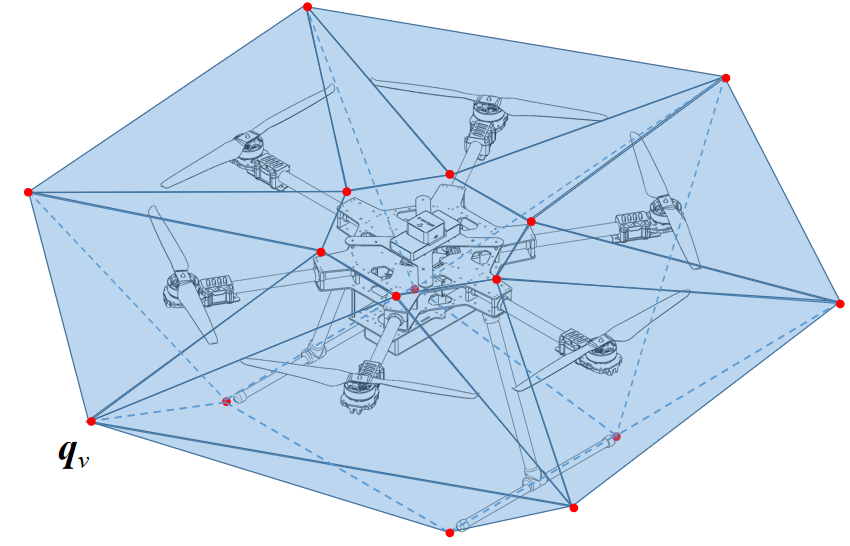
\includegraphics[width = 0.62\textwidth]{approximate_polyhedron.png}
  \caption{用凸多面体近似飞行器的形状}
  \label{fig:using_polyhedron_to_approximate_geometry_of_drone}
\end{figure}

由凸集的性质,飞行器整体包含在安全飞行走廊内等价于长方体的8个顶点全部在安全飞行走廊内,
因此如\figref{fig:using_polyhedron_to_approximate_geometry_of_drone}所示,其实可以将飞行器的形状用任意合适形状的凸多面体近似\cite{2021Fast}。
长方体8个顶点在机体坐标系$\mathscr{F}_b$下的坐标为:
\begin{equation}
  \hat{\bm{q}}_v = \trans{
    \begin{bmatrix}
      \pm\frac{l_x}{2} & \pm\frac{l_y}{2} & \pm\frac{l_z}{2} 
    \end{bmatrix}
  }, v = 1, 2, \cdots, 8
  \label{equ:vertices_of_cuboid_in_body_frame}
\end{equation}
则轨迹上$t$时刻这8个顶点在世界坐标系$\mathscr{F}_W$下的坐标为:
\begin{equation}
  \bm{q}_v(t) = \bm{p}(t) + \bm{R}(\bm{\sigma}(t))\hat{\bm{q}}_v ,
  v = 1, 2, \cdots, 8
  \label{equ:vertices_of_cuboid_in_world_frame}
\end{equation}
其中$\bm{R}(\bm{\sigma}(t))$二阶连续可微。

在优化过程中,我们把每段轨迹都约束到到一个凸多面体中,第$i$段轨迹所在的凸多面体用H-表示法用线性不等式约束表示为:
\begin{equation}
  \mathcal{P}_i = 
  \left\{
      \bm{p} \in \mathbb{R}^3 \mid \bm{a}_{i,k}^{\text{T}}\bm{p}-b_{i,k} \leq 0, \left\| \bm{a}_{i,k} \right\|_2=1, k=1,2,\cdots,K_i
  \right\}
  \label{equ:ith_piece_s_polyhedron}
\end{equation}
接下来就可以根据\cite{yang2021whole}的思想构造出关于$SE(3)$安全约束的时间积分碰撞惩罚:
\begin{equation}
  E_c = W_c  \sum_{i=1}^M \int_{t_{i-1}}^{t_i} \sum_{v=1}^8 \sum_{k=1}^{K_i} \mathcal{K}(\bm{a}_{i,k}^{\text{T}}\bm{q}_v(t) - b_{i,k}) \mathrm{d}t 
  \label{equ:collision_penalty}
\end{equation}
将\equref{equ:velocity_penalty}、\equref{equ:acceleration_penalty}、\equref{equ:angular_velocity_penalty}和\equref{equ:collision_penalty}用矩形法则进行近似得:
\begin{align}
  &E_v \approx I_v(\bm{c}, \bm{T}) = W_v \sum_{i=1}^M \sum_{j=1}^{\kappa} \mathcal{K}(\left\|\dot{\bm{p}}(t_{i-1}+\frac{j}{\kappa}T_i)\right\|_2^2 - v_{max}^2)\frac{T_i}{\kappa}
  \label{equ:velocity_penalty_approx}\\
  &E_a \approx I_a(\bm{c}, \bm{T}) = W_a \sum_{i=1}^M \sum_{j=1}^{\kappa} \mathcal{K}(\left\|\ddot{\bm{p}}(t_{i-1}+\frac{j}{\kappa}T_i)\right\|_2^2 - a_{max}^2)\frac{T_i}{\kappa}
  \label{equ:acceleration_penalty_approx}\\
  &E_{\omega} \approx I_{\omega}(\bm{c}, \bm{T}) = W_{\omega} \sum_{i=1}^M \sum_{j=1}^{\kappa} \mathcal{K}(\left\|\bm{\omega}(t_{i-1}+\frac{j}{\kappa}T_i)\right\|_2^2 - {\omega}_{max}^2)\frac{T_i}{\kappa}
  \label{equ:acceleration_penalty_approx}\\
  &E_c \approx I_c(\bm{c}, \bm{T}) = W_c  \sum_{i=1}^M \sum_{j=1}^{\kappa} \sum_{v=1}^8 \sum_{k=1}^{K_i} \mathcal{K}(\bm{a}_{i,k}^{\text{T}}\bm{q}_v(t_{i-1}+\frac{j}{\kappa}T_i) - b_{i,k})\frac{T_i}{\kappa}
  \label{equ:collision_penalty_approx}
\end{align}

下面求取上述罚函数关于$\bm{c}$和$\bm{T}$的梯度。
观察罚函数的结构,其由一系列关于$\mathcal{K}(\cdot) = \max(\cdot, 0)^3$的项求和得到,
我们只需计算每个求和项为正,即超出约束部分的梯度;对于约束满足的部分,对应梯度则为0。我们令:
\begin{align}
  & I_{v_{ij}} = W_v (\left\|\bm{v}\right\|_2^2 - v_{max}^2)^3\frac{T_i}{\kappa}
  \label{equ:Evij}\\
  & I_{a_{ij}} = W_a (\left\|\bm{a}\right\|_2^2 - a_{max}^2)^3\frac{T_i}{\kappa}
  \label{equ:Eaij}\\
  & I_{\omega_{ij}} = W_{\omega} (\left\|\bm{\omega}\right\|_2^2 - \omega_{max}^2)^3\frac{T_i}{\kappa}
  \label{equ:Eoij}\\
  & I_{c_{ijvk}} = W_c(\bm{a}_{i,k}^{\text{T}}\bm{q}_v - b_{i,k})^3\frac{T_i}{\kappa}
  \label{equ:Ecijvk}
\end{align}
其中$\bm{v},\bm{a},\bm{\omega},\bm{q}_v$和$\bm{R}$为$t=t_{i-1}+\frac{j}{\kappa}T_i$时的取值。
则\equref{equ:Evij}、\equref{equ:Eaij}、\equref{equ:Eoij}和\equref{equ:Ecijvk}分别关于$\bm{c}$和$\bm{T}$的梯度见附录\ref{appdx:A}。

由于旋转矩阵$\bm{R}$和角速度$\bm{\omega}$等与姿态有关的量与$\bm{\sigma}$紧密相关,
故上述罚函数正向求值和反向求梯度的过程会因姿态参数化方法的不同而不同。
可以选取各种合理的姿态参数化方法来规划姿态轨迹$\bm{\sigma}(t)$,只要使$\bm{R}$和$\bm{\omega}$等姿态相关量关于$\bm{\sigma}$二阶连续可微即可,
不同的姿态参数化方法给轨迹优化问题\equref{equ:final_unconstrained_optimization_problem}所带来的差异将只体现在惩罚项$I_\Sigma$中。

\subsection{基于欧拉角姿态表示的过驱动飞行器$SE(3)$轨迹生成}\label{subsec:planning_based_on_euler_angle}
本小节采用ZYX欧拉角来表示姿态,即取轨迹$\bm{z}(t)$的姿态部分$\bm{\sigma}(t)$为:
\begin{equation}
  \bm{\sigma}(t) = \bm{\varepsilon}(t) = 
  \begin{bmatrix}
    \phi(t) \\ \theta(t) \\ \psi(t)
  \end{bmatrix}
\end{equation}
则旋转矩阵$\bm{R}$和角速度$\bm{\omega}$可表示为: 
\begin{gather}
  \bm{R}(\bm{\sigma}) = \bm{R}(\bm{\varepsilon}) = 
  \begin{bmatrix}
    \cos\o\psi\cos\theta & & \cos\psi\sin\theta\sin\phi - \sin\psi\cos\phi & & \cos\psi\sin\theta\cos\phi + \sin\psi\sin\phi \\
    \sin\psi\cos\theta & & \sin\psi\sin\theta\sin\phi + \cos\psi\cos\phi & & \sin\psi\sin\theta\cos\phi - \cos\psi\sin\phi \\
    -\sin\theta & & \cos\theta\sin\phi & & \cos\theta\cos\phi
  \end{bmatrix} \label{equ:euler_angle_to_R}\\
  \bm{\omega}(\bm{\sigma}, \dot{\bm{\sigma}}) = \bm{\omega}(\bm{\varepsilon}, \dot{\bm{\varepsilon}}) = 
  \bm{W}\dot{\bm{\varepsilon}} = 
  \begin{bmatrix}
    \dot{\phi}\cos\theta - \dot{\psi}\cos\phi\sin\theta \\ 
    \dot{\theta} + \dot{\psi}\sin\phi \\ 
    \dot{\phi}\sin\theta + \dot{\psi}\cos\phi\cos\theta
  \end{bmatrix} \label{equ:euler_angle_to_omega}
\end{gather}
式中$\bm{W}$是欧拉角速率到世界坐标系下机体角速度$\bm{\omega}$的变换矩阵,其表达形式为:
\begin{equation}
  \bm{W} = 
  \begin{bmatrix}
    \cos\theta & & 0 & & -\cos\phi\sin\theta \\ 
    0 & & 1 & & \sin\phi \\
    \sin\theta & & 0 & & \cos\phi\cos\theta
  \end{bmatrix}
  \label{equ:W}
\end{equation}

$\bm{R}$与$\bm{\omega}$关于$\bm{c}$和$\bm{T}$的梯度具有解析的表达式,详见附录\ref{appdx:B}。

\subsection{基于四元数姿态表示的过驱动飞行器$SE(3)$轨迹生成}\label{subsec:planning_based_on_quaternion}
四元数是刚体姿态表示的一种常见形式。
与欧拉角表示法的主要区别在于,四元数表示法不存在奇异性,同一个姿态有且仅有两个单位四元数与之对应,且这两个单位四元数互为加法逆元。

Terzakis等人提出过利用球极投影参数化四元数的方式\cite{terzakis2014quaternion}。
以单位四元数超球面的一个极点$\bm{Q}_0=\trans{[1\  0 \ 0 \ 0]}$作球极投影,
就在除去该极点的超球面与整个$\mathbb{R}^3$空间建立了一个连续光滑的双射,
该映射的逆映射的表达式为: 
\begin{equation}
  \bm{Q} = \bm{Q}(\bm{\varrho}) = \trans{
    \begin{bmatrix}
      \frac{\trans{\bm{\varrho}}\bm{\varrho}-1}{\trans{\bm{\varrho}}\bm{\varrho}+1} & 
      \frac{2\trans{\bm{\varrho}}}{\trans{\bm{\varrho}}\bm{\varrho}+1}
    \end{bmatrix}
  } \in SO(3), \forall \bm{\varrho} \in \mathbb{R}^3
  \label{equ:R3_to_quaternion}
\end{equation}

显然用$\bm{\varrho}$作为姿态的参数化表示是满足二阶连续可微的条件的,
因此平坦输出轨迹也可以表示为:
\begin{equation}
  \bm{\sigma}(t) = \bm{\varrho}(t)
\end{equation}

旋转矩阵和角速度用单位四元数$\bm{Q} = \trans{[w\  x \ y \ z]}$表示为:
\begin{gather}
  \bm{R}(\bm{Q}) = 
  \begin{bmatrix}
    1 - 2y^2 -2z^2 & & 2(xy - wz) & & 2(xz + wy) \\ 
    2(xy + wz) & & 1 - 2x^2 - 2z^2 & & 2(yz - wx) \\ 
    2(xz - wy) & & 2(yz + wx) & & 1 - 2x^2 - 2y^2
  \end{bmatrix} \label{equ:quaternion_to_R} \\ 
  \bm{\omega} = 2\bm{U}\dot{\bm{Q}} = 2\bm{U}\trans{\bm{G}}\dot{\bm{\varrho}} \label{equ:dquat_to_omega}
\end{gather}
其中: 
\begin{gather}
  \bm{U} = 
  \begin{bmatrix}
    -x & & w & & -z & & y \\
    -y & & z & & w & & -x \\
    -z & & -y & & x & & w
  \end{bmatrix} \in \mathbb{R}^{3\times 4} \label{equ:matrix_U}\\
  \bm{G} = 
  \begin{bmatrix}
    \pdiff{w}{\bm{\varrho}} & & \pdiff{x}{\bm{\varrho}} & & \pdiff{y}{\bm{\varrho}} & & \pdiff{z}{\bm{\varrho}}
  \end{bmatrix} \in \mathbb{R}^{3 \times 4} \label{equ:matrix_G}
\end{gather}
$\bm{G}$以及罚函数梯度的具体形式详见附录\ref{appdx:C}。

\subsection{算法实现}\label{subsec:impl_of_traj_opt_algo}
\subsubsection{中间点分配与初始中间点确定}
由一系列凸多面体$\{\mathcal{P}^1,\cdots,\mathcal{P}^{M_\mathcal{P}}\}$组成的飞行走廊一定满足如下条件:
\begin{equation}
  \begin{cases}
    \mathcal{P}^i \cap \mathcal{P}^j = \emptyset, \quad \vert i-j \vert = 2 \\
    \text{Int}(\mathcal{P}^i \cap \mathcal{P}^j) \neq \emptyset, \quad \vert i-j \vert \leq 1
  \end{cases}
  \label{equ:conditions_of_sfc}
\end{equation}
且起始位置点和终止位置点一定分别在凸多面体$\mathcal{P}^1$和$\mathcal{P}^{M_\mathcal{P}}$内。
根据\equref{equ:spatial_constraints_minco},每个位置中间点都会硬性约束在一个凸多面体中,
通常的中间点分配策略是:在每两个相邻的凸多面体的相交区域内部$\text{Int}(\mathcal{P}^{i-1} \cap \mathcal{P}^i)$内分配一个位置中间点,
在此将这样的位置点以及起始位置点和终止位置点统称为关键点;
随后在相邻两个关键点之间分配若干个位置中间点到$\mathcal{P}^{i-1}$中。

\begin{figure}[ht]
  \centering
  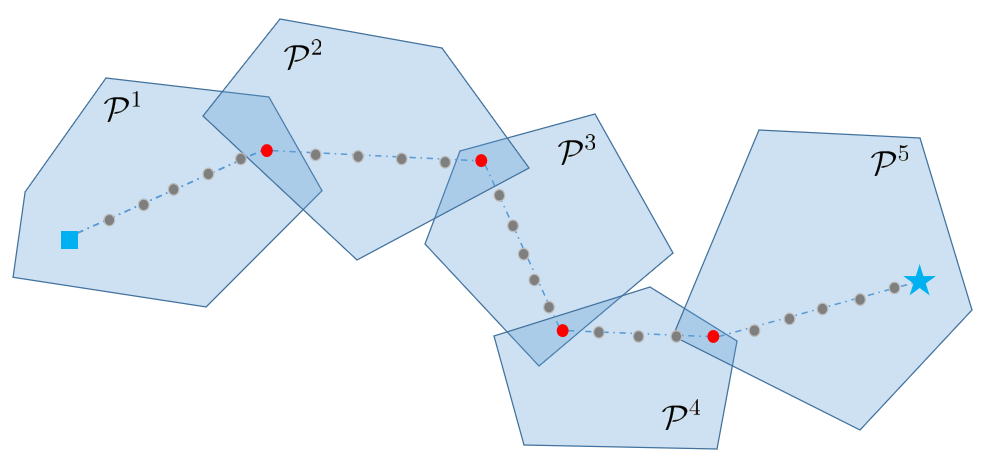
\includegraphics[width = 0.8\textwidth]{assign_initial_q.png}
  \caption{初始位置中间点分配示意图}
  \label{fig:assign_initial_q}
\end{figure}

根据以上信息,在本课题的实现中初始中间点分配方法如下:
\begin{enumerate}
  \renewcommand{\labelenumi}{(\theenumi)}
  \item 在相邻两个凸多面体的交集内部$\text{Int}(\mathcal{P}^{i-1} \cap \mathcal{P}^i)$中分配一个位置关键点(\figref{fig:assign_initial_q}中的红色点),
  这个步骤通过将位置点在$\text{Int}(\mathcal{P}^{i-1} \cap \mathcal{P}^i)$中的重心坐标设为$1/(n_g+1)$来实现,
  由凸多面体的H-表示法枚举其顶点的算法使用开源方案\footnote{https://github.com/ZJU-FAST-Lab/VertexEnumeration3D};
  \item 在相邻两个位置关键点之间以一定间距作线性插值得到一系列分配到$\mathcal{P}^{i-1}$中的位置中间点(\figref{fig:assign_initial_q}中的灰色点);
  \item 所有中间点的初始姿态分量均设为$\textbf{0}$
\end{enumerate}

\subsubsection{时间正则项与微分同胚映射选取}
如\equref{equ:final_form_of_time_regularized_control_effort}所示, 
本优化器不固定轨迹总时间,且时间正则项与总时间成正比,也就是说优化时会倾向于使轨迹更快地到达终点;
此外,本课题在实现优化器时使用的时间约束消去微分同胚变换并非指数函数,而是参考GCOPTER官方实现\footnote{https://github.com/ZJU-FAST-Lab/GCOPTER}使用下述形式的微分同胚映射:
\begin{equation}
  T_i = 
  \begin{cases}
    1 + \tau_i(0.5\tau_i + 1), \quad \tau_i > 0 \\
    {1}/(1 + \tau_i(0.5\tau_i - 1)), \quad \tau_i \leq 0
  \end{cases}
  \label{equ:the_actual_diffeomorphism_used}
\end{equation}

\subsubsection{自定义约束的接口}
为了提高优化器的复用性、充分发挥几何约束优化器灵活性的优点,对于自定义约束$\mathcal{G}$,
在实际实现时将时间积分罚函数抽象为了SE3TimeIntPenalty类,提供evaluate()公共接口,
此接口返回罚函数值及其关于$\bm{c}$和$\bm{T}$的梯度,
当面对不同的任务需求时,只需继承SE3TimeIntPenalty类,用需求对应的罚函数重写evaluate()接口,并与优化器关联即可。

\subsubsection{优化算法实现}
在实现中采用L-BFGS算法\cite{liu1989limited}作为无约束优化算法,Wang有开源的算法实现\footnote{https://github.com/ZJU-FAST-Lab/LBFGS-Lite},
但其中仅使用Lewis等人提出的线搜索方法\cite{lewis2013nonsmooth},该方法若在一定迭代次数后不能找到满足条件的点则视为线搜索失败,随之整个优化过程也宣告失败;
受限于计算机对极小数字的分辨能力,在本课题这种目标函数数值特性不太好的情况下就很难优化成功。
于是本课题在重新实现一遍L-BFGS算法的同时,使用的线搜索策略变为:若某次Lewis线搜索失败,则使用Backtracking法,
这样可确保优化过程不会因为线搜索失败而中断。

本课题中上述优化器使用C++17标准实现。

\section{本章小结}\label{sec:summary_4}
本章首先详细介绍了几何约束下多旋翼飞行器轨迹优化框架的基本原理,
给出了其基本问题形式、重要技巧等;
随后根据过驱动飞行器的特点,结合几何约束优化的核心思想,
确定了适用于过驱动飞行器6自由度$SE(3)$轨迹优化的问题形式,
并给出了相关公式的推导,设计出了几何约束下过驱动飞行器轨迹优化的算法框架;
最后给出了基于欧拉角和基于四元数的两种适用于本框架的姿态参数化方式。

本章完成了过驱动飞行器轨迹规划后端部分的算法设计。
至此,一个完整的过驱动飞行器轨迹规划框架设计完毕。

